\begin{figure}[h!tbp]{\textwidth}
  \centering
  \caption{Hopfiel Network diagram.}%
  \label{fig:hopfield-diagram}%
  \tikzstyle{visible} = [draw, circle, fill=white]
  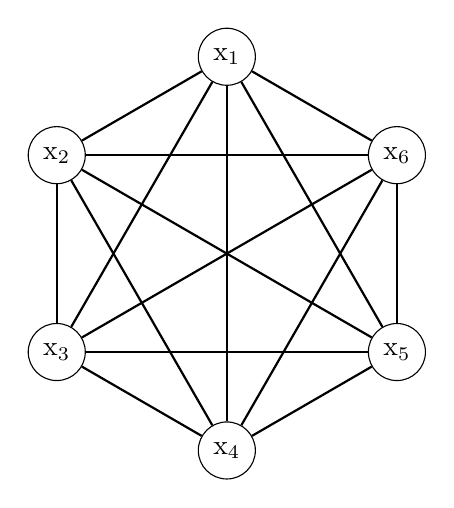
\begin{tikzpicture}
    \node[style=visible] (a) at (0, 2.5) {$\mathrm{x}_{1}$};
    % \node[style=visible] (b) at +(0: 1.5) {$\mathrm{x}_{2}$};
    % \node[style=hidden] (c) at + (60: 1.5) {$\mathrm{x}_{3}$};
    \node[style=visible] (b) at (-2.16, 1.25) {$\mathrm{x}_{2}$};
    \node[style=visible] (c) at (-2.16, -1.25) {$\mathrm{x}_{3}$};
    \node[style=visible] (d) at (0, -2.5) {$\mathrm{x}_{4}$};
    \node[style=visible]  (e) at (2.16, -1.25) {$\mathrm{x}_{5}$};
    \node[style=visible]  (f) at (2.16, 1.25) {$\mathrm{x}_{6}$};
    \foreach \from/\to in {a/b, a/c, a/d, a/e, a/f, b/c, b/d, b/e, b/f, c/d, c/e, c/f, d/e, d/f, e/f}
      \draw [thick] (\from) -- (\to);   
  \end{tikzpicture}
  \legend{Each white circle represents a single unit of the Hopfield Network.}
  \source{Author.}
\end{figure}
